\subsection{Music recommendation}
Collaborative filtering is the part of recommender systems that predicts users' preferences for particular items. The major challenge in predicting users'listening counts, as in our task, is that the available user-artist entries are usually too few and sometimes a method's performance relies on a good initial estimation of the unknown entries. 
We therefor decided to implement besides the common KNN, Kmeans also ALS[cite here], which uses only the known listening counts and avoids dependency on initial estimations.

\subsection{Data description}
The training data consists in a matrix $Ytrain$ of size $1774$x$15082$, corresponding to $1774$ users and $15802$ artists. Entry $Ytrain(i,j)$ expresses how many times user $i$ has listened to artist $j$. An entry of 0 means we do not have information for that $(user, artist, count)$ triple.
We are also given the friendship graph of the $1774$ users stored as an adjacency matrix.

\subsection{Exploratory Data Analysis}

The matrix $Ytrain$ is very sparse with a density of only $0.0026\%$, corresponding to 
$69617 (user, artist, count)$ triples. 
The variance of the entries' values is very high, the maximum  being $352698$ and average listening count per user and per artist of 5.52 and 5.46 respectively. There were also 1262 artists for which no information was provided.

A histogram of all the listening counts, shown in Fig\ref{fig:count_distribution} $a)$ tells us that the known entries follow a heavy tail distribution. The long tail contains a small number of popular items, the well-known artists, and the rest are located in the heavy tail.
One method to transform skewed data such that it becomes more gaussian distributed is to use the Box-Cox transform
\\
\begin{table}[h]
  \centering
  \begin{tabular}{c  c }
  $data(\lambda)$&= $log(data), \lambda = 0$ \\ 
                            &= $\frac{data^\lambda - 1}{\lambda} ,\lambda \neq 0$ \\ 
  \end{tabular}
\end{table}

In our case, we can choose $\lambda=0$ because our values are very high and positive. This transformation will make the distances between listening counts much smaller and will reduce the influence on error of the (user,artist,count) triples in the long tail. 

The results after data transformation can be seen in Fig \ref{fig:user_artist_distribution}. The distribution of the user counts and of the artist counts are closer to a normal distribution. We notice there are some far away entries with values greater than 14. These will have a higher impact on the untransformed data. An off by 1 error here will have more impact than on the small entries.

\begin{figure}[h]
  \centering
  \begin{subfigure}[b]{0.45\textwidth}
   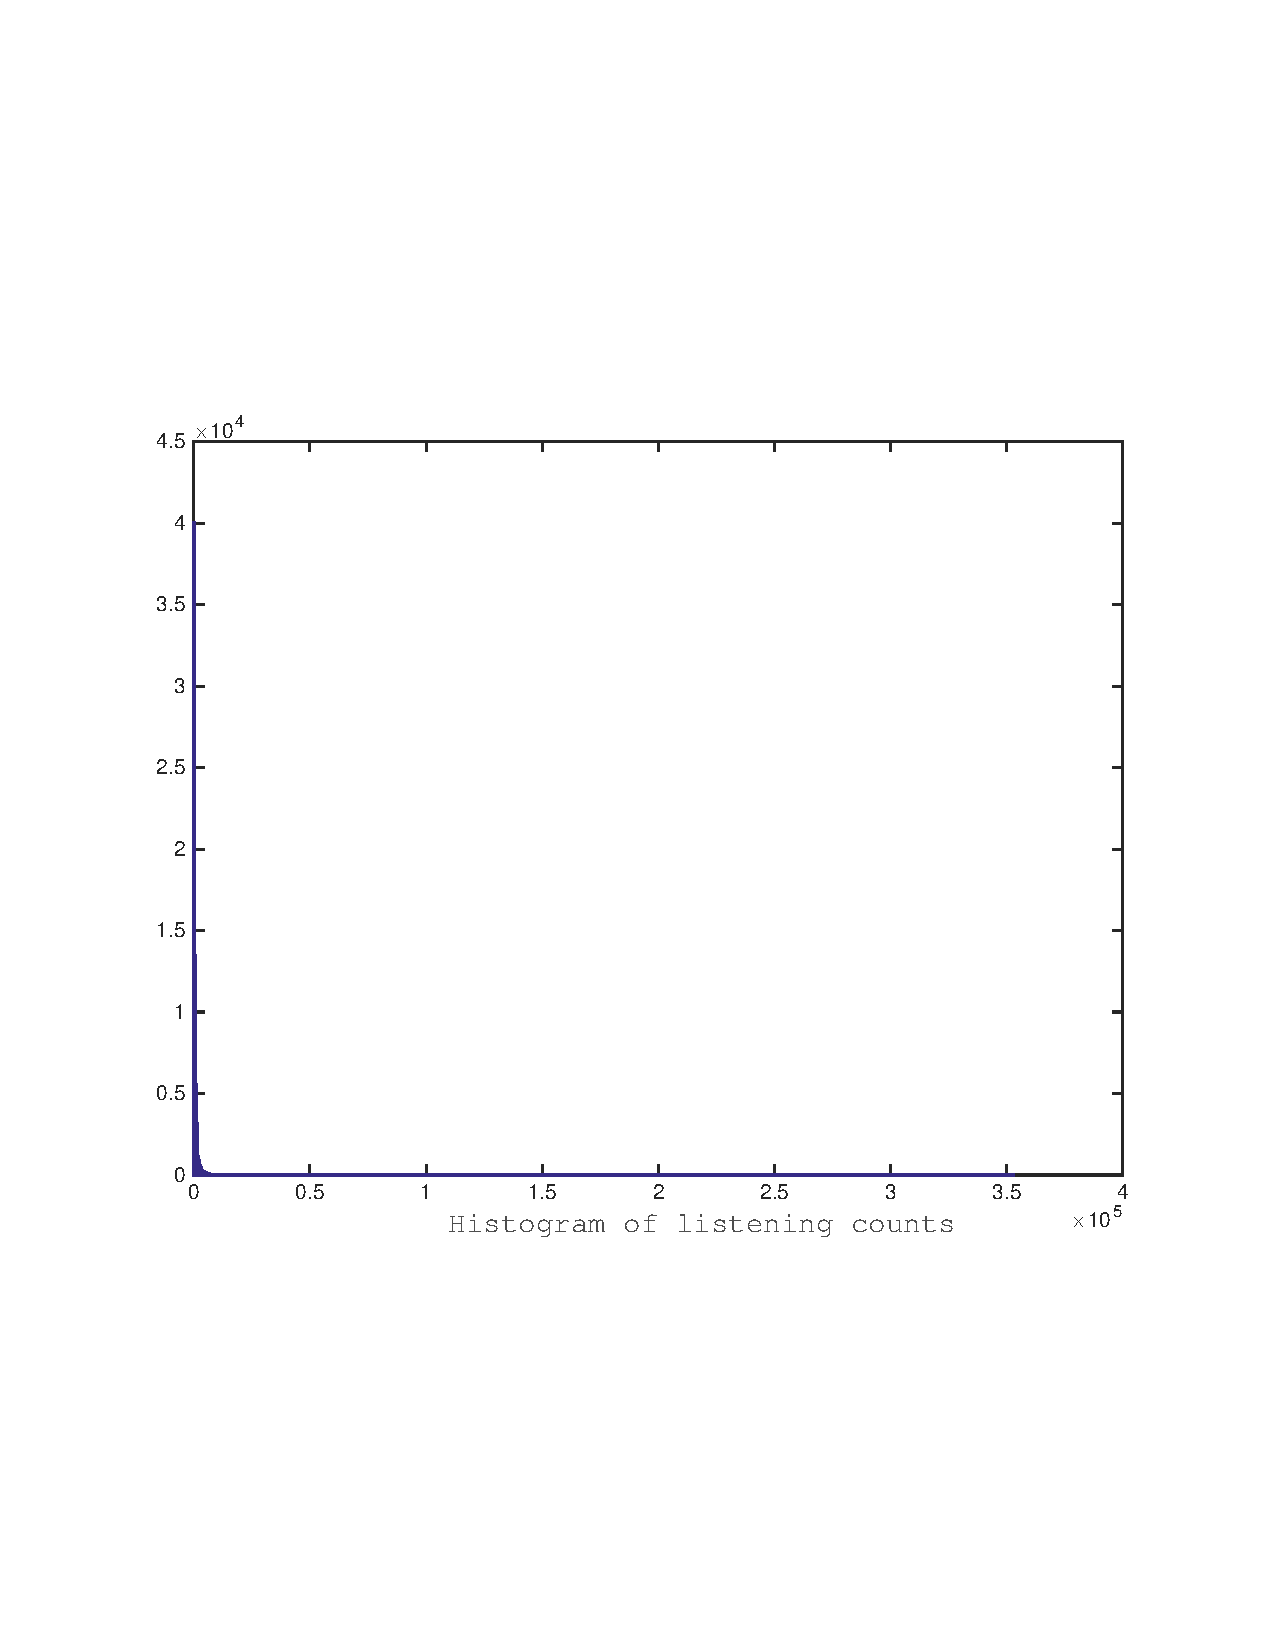
\includegraphics[width=\textwidth]{figures/histYtrain_crop.pdf}
    \caption{Before data transformation}
  \end{subfigure}
  \begin{subfigure}[b]{0.45\textwidth}
    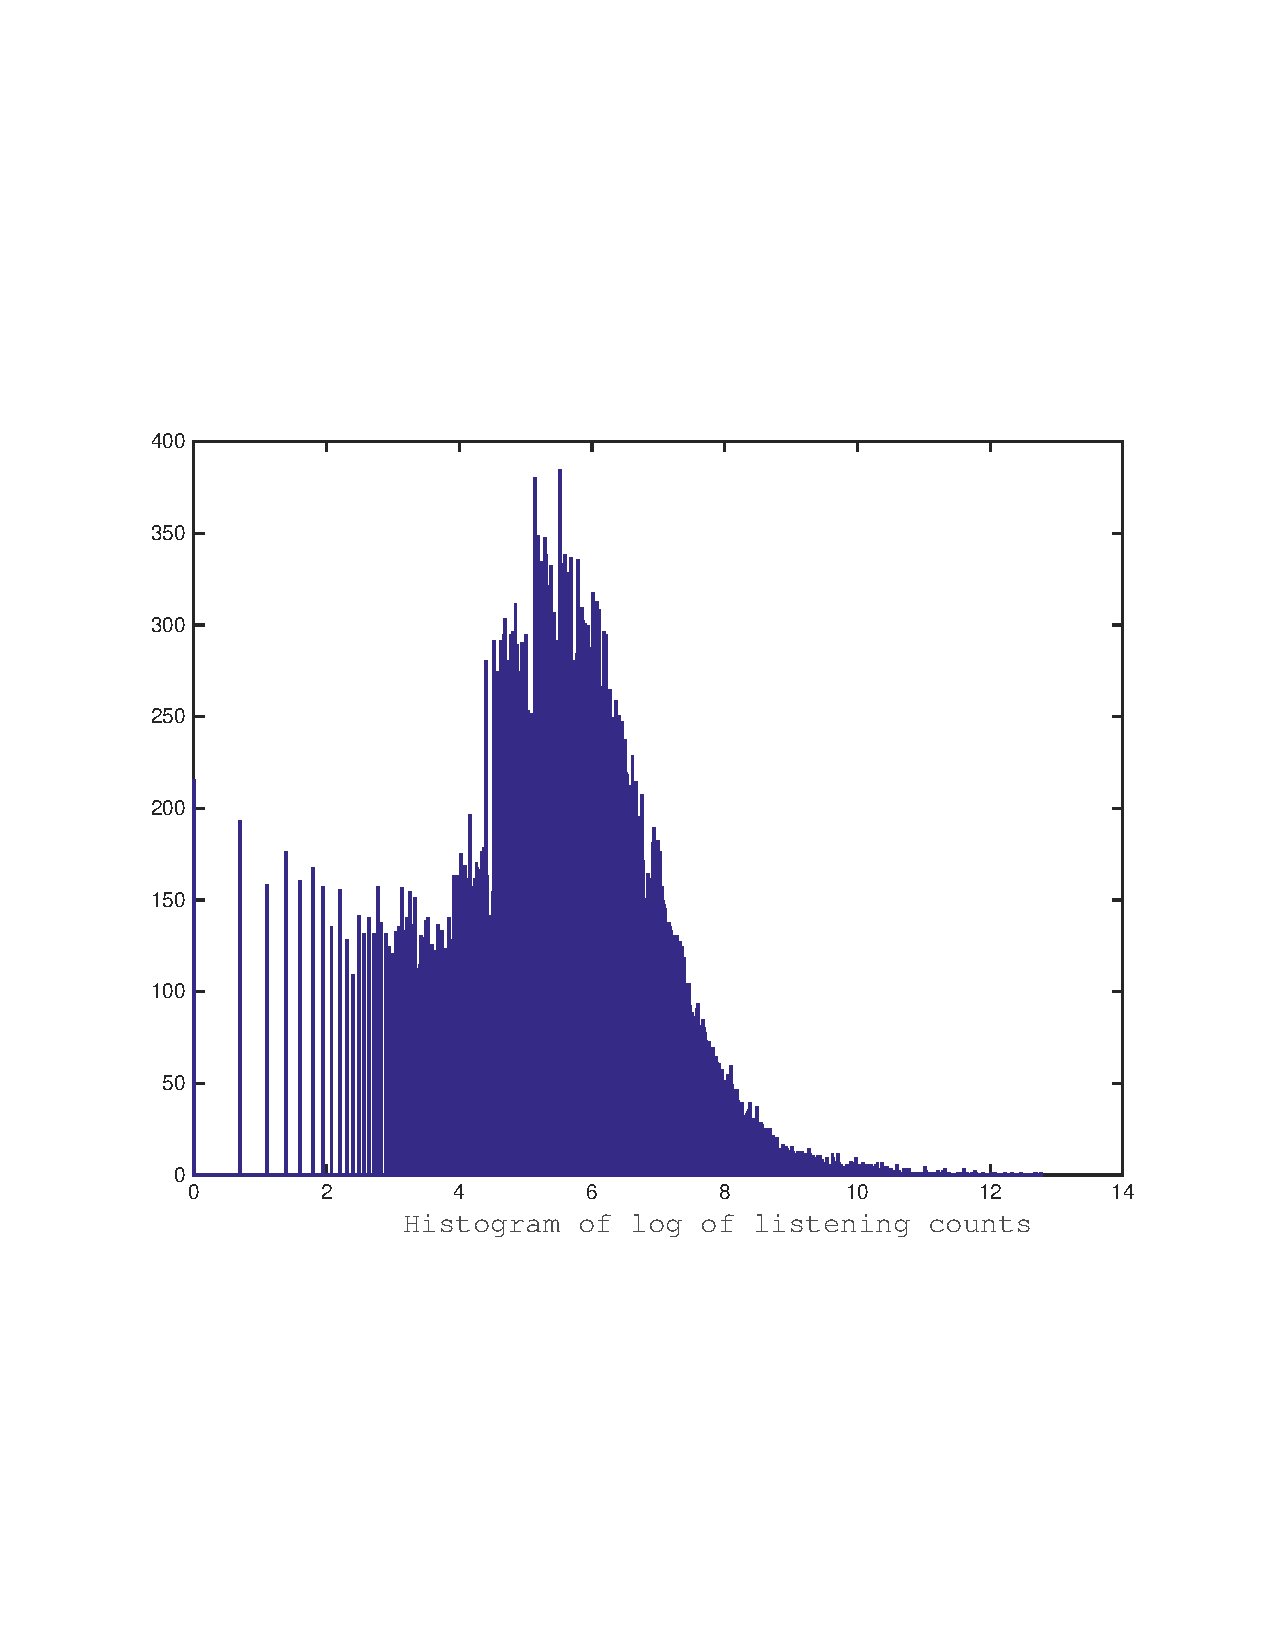
\includegraphics[width=\textwidth]{figures/histLogYtrain_crop.pdf}
    \caption{After data transformation}
  \end{subfigure}
  \caption{Distribution of all listening counts}
  \label{fig:count_distribution}
\end{figure}

\begin{figure}[h]
  \centering
  \begin{subfigure}[b]{0.45\textwidth}
   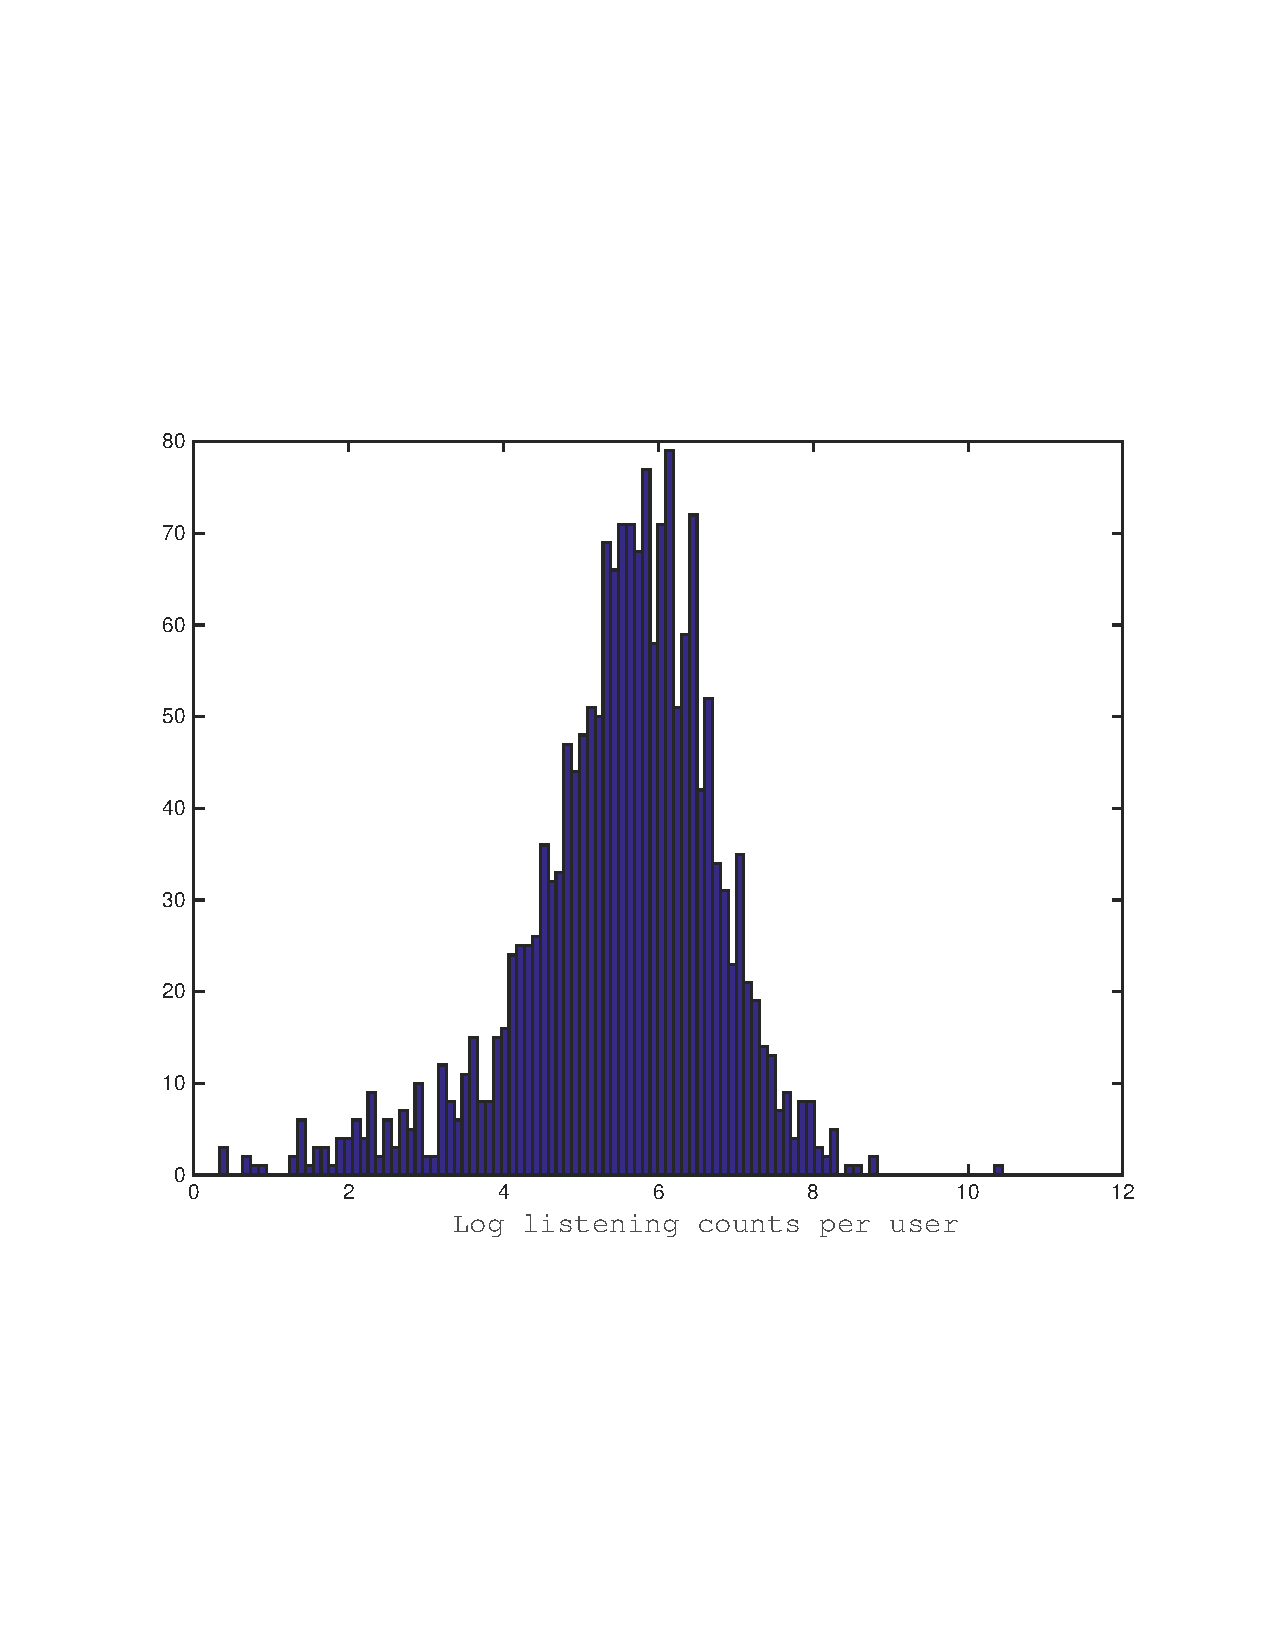
\includegraphics[width=\textwidth]{figures/histCountPerUser.pdf}
    \caption{}
  \end{subfigure}
  \begin{subfigure}[b]{0.45\textwidth}
    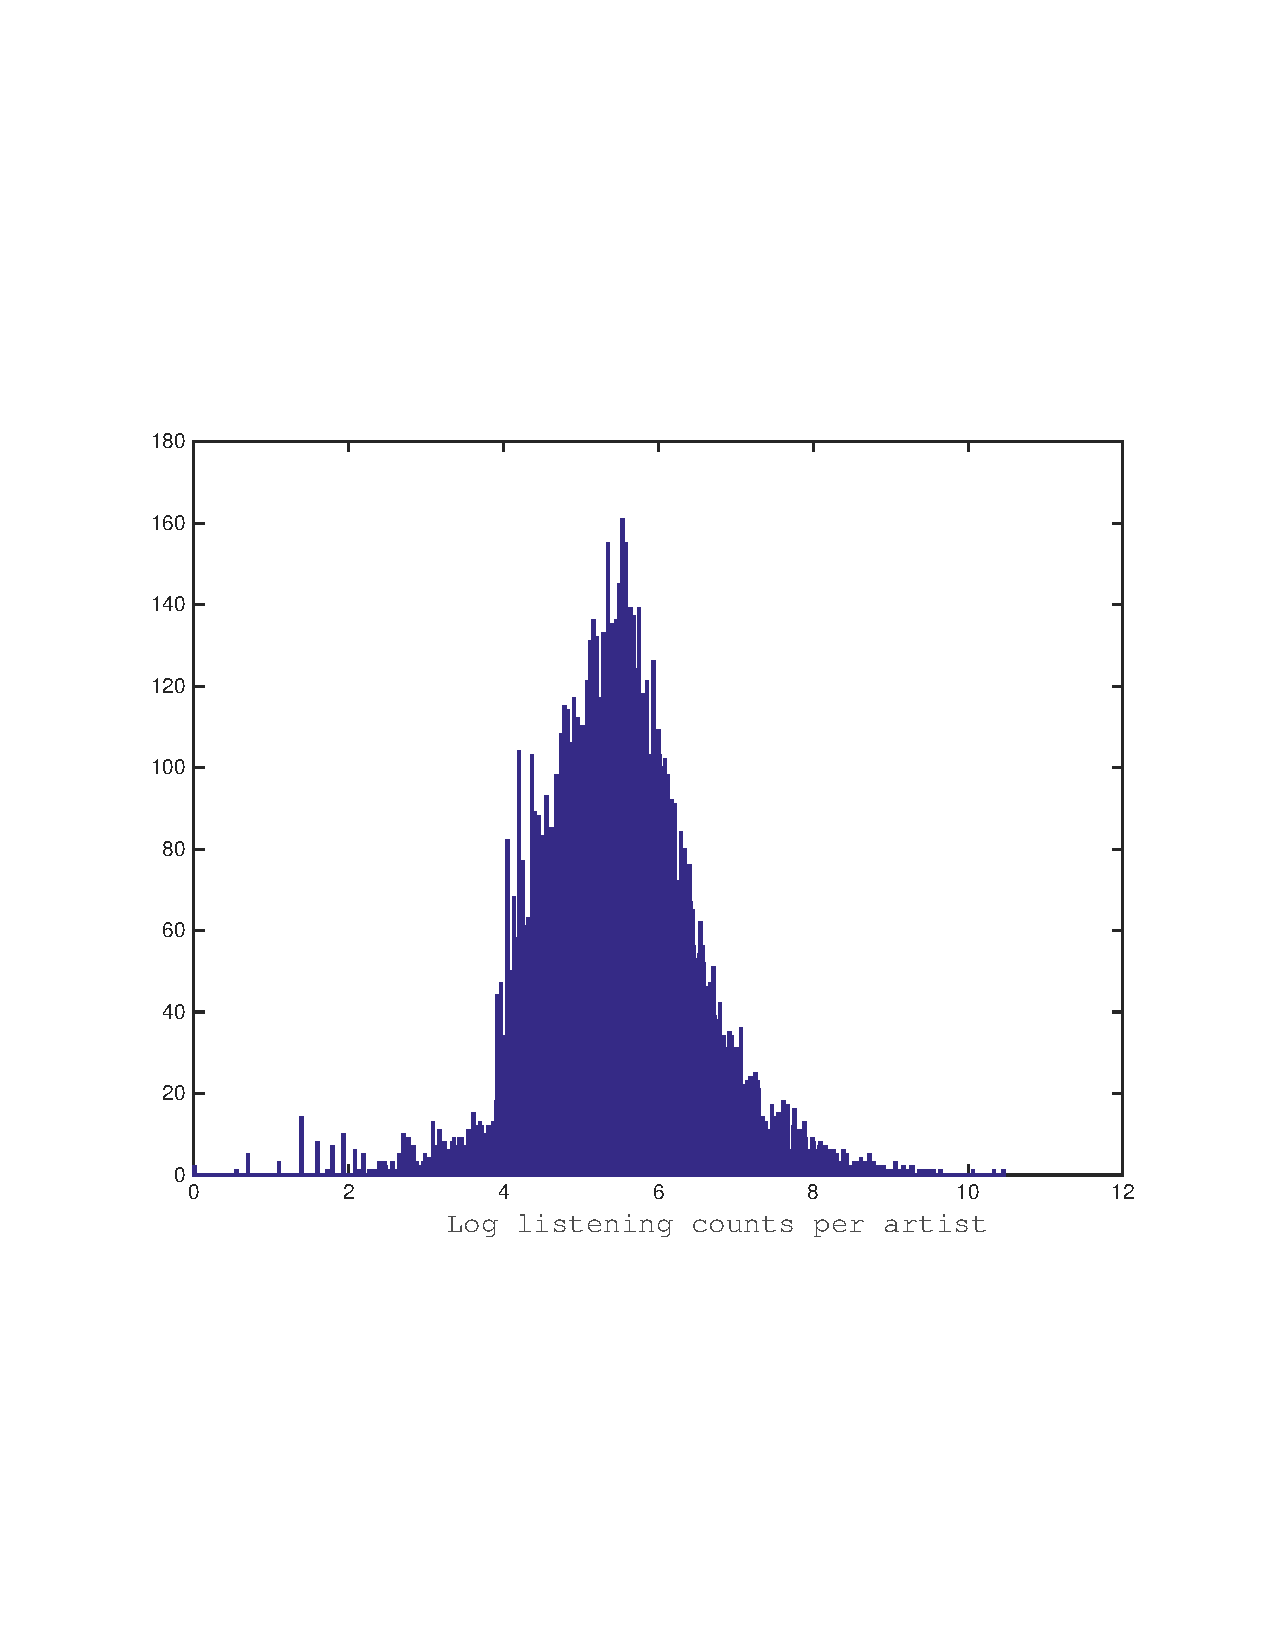
\includegraphics[width=\textwidth]{figures/histCountPerArtist.pdf}
    \caption{}
  \end{subfigure}
  \caption{Distribution per user (a) and per artist (b) log of listening count distribution}
  \label{fig:user_artist_distribution}
\end{figure}

 
\subsection{Task 1}
In all our experiments we used 10-fold cross validation and repeated the experiments twice.
For the first task, we randomly omit 10 entries for every artist.
Splitting the data was more difficult since we needed to make sure we do not
remove all the entries for an artist. If an artist has $m$ entries with $m < 10$, then we keep $m-1$ entries for testing,
 to still have one element for training.
 
 
\subsection{Baseline}
There are three simple basic predictions one can try: the global average count, the average count per user and the average count
per artist prediction. All of these methods give similar MAE results:  1.1117($pm$ 0.0079), 0.64($pm$ 0.0042) and   1.2134($pm$ 0.0092).
We note that the final MAE is composed of various values, small and large. In Fig we can see a ploto of the MAE error terms in log format.

\subsubsection{KNN}
\textcolor{red}{TODO}


\subsubsection{ALS}
We do not review here the details of ALS algorithm, the reader can consult the paper[cite] beforehand, since this was not the goal of this report.
\textcolor{red}{TODO}

Using 20 features and $lambda in [0.01,0.05,0.1,0.5,1]$ we obtain the results in table \ref{table:labda_choice} using 10-fold cross validation. The experiments were repeated twice with different seed. We note that we stopped the update steps in the algorithm only after 5 iterations because the update step was very computational intensive.

\begin{minipage}{\textwidth}
  \begin{minipage}[b]{0.45\textwidth}
    \centering
    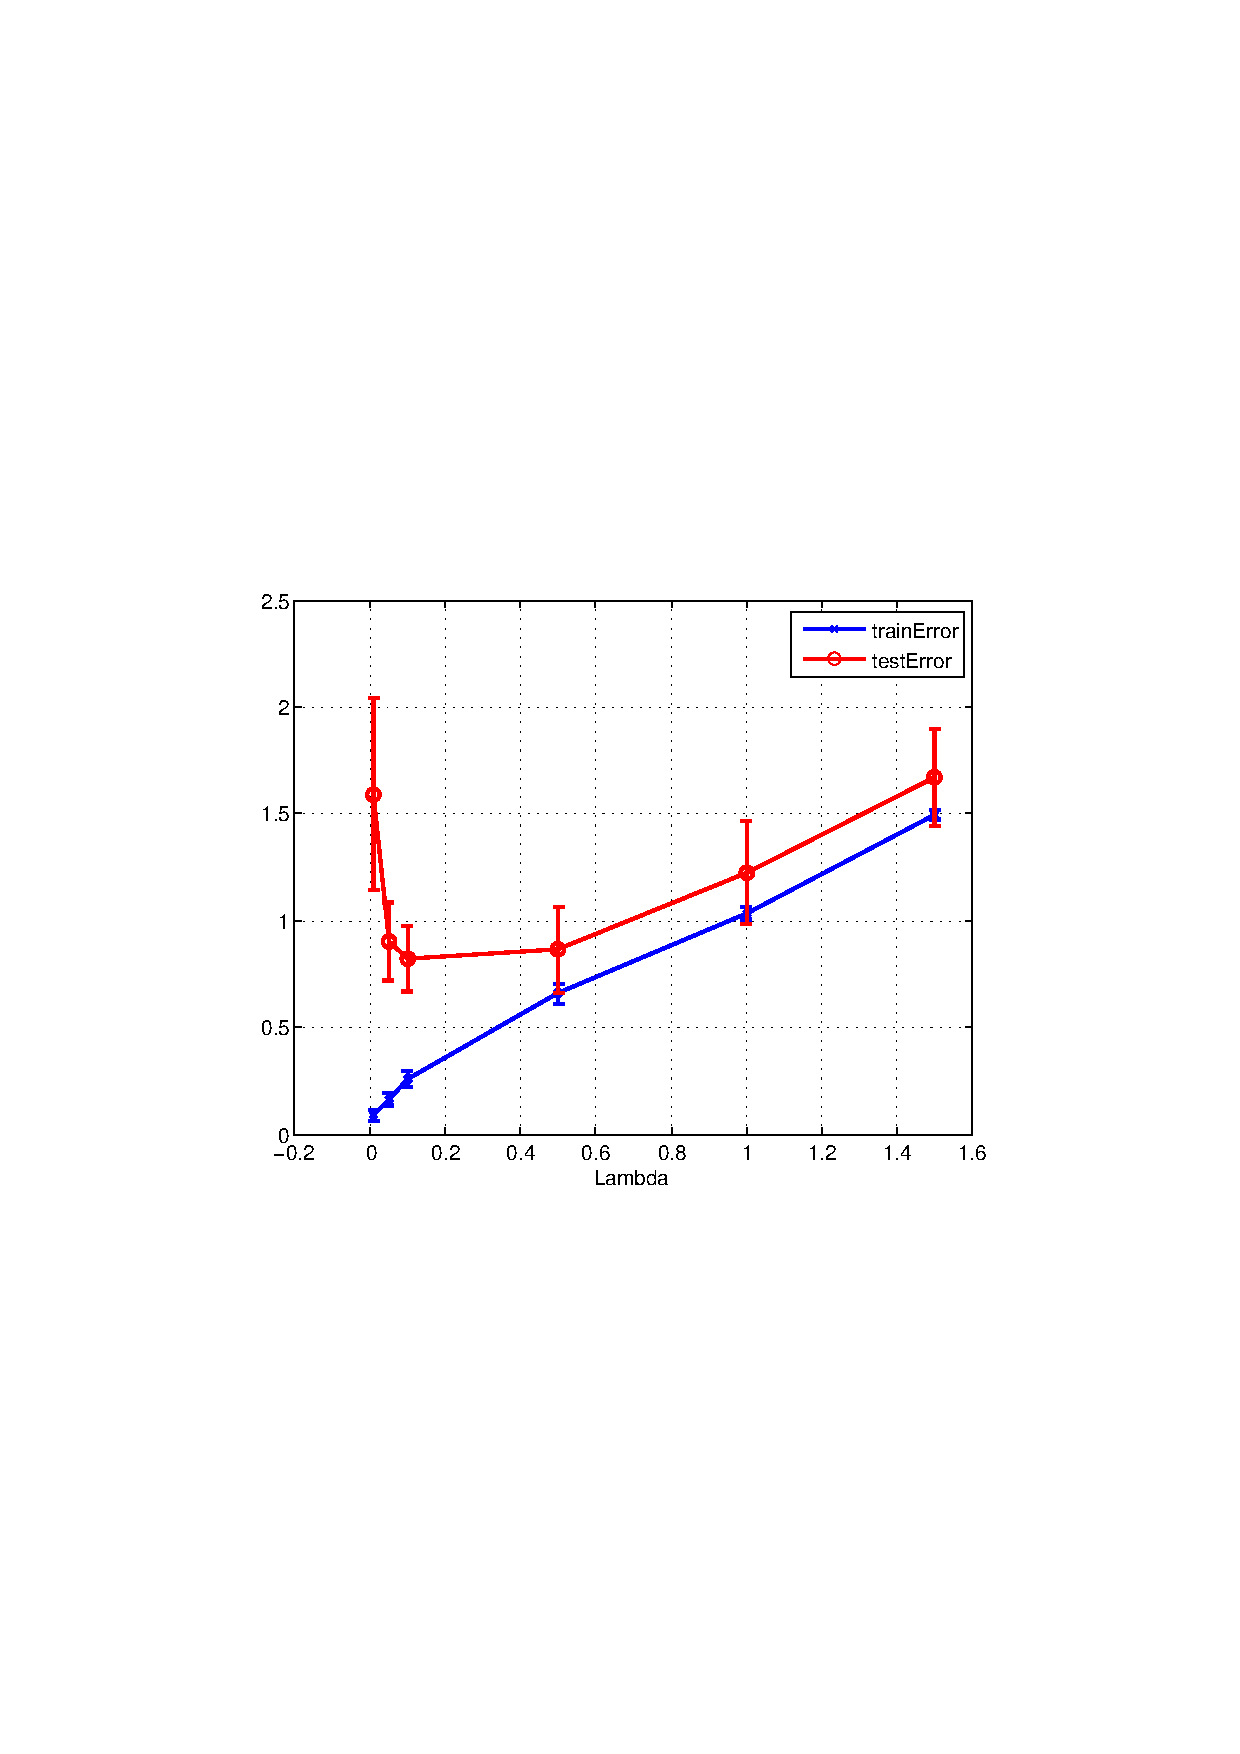
\includegraphics[clip, trim=4cm 9.2cm 3.5cm 9cm, width=\textwidth]{figures/ALS_lambda.pdf}
    \captionof{figure}{Comparison of Train and Test errors with different lambda values}
    \label{fig:ALS_lambdas}
  \end{minipage}
  \hfill
  \begin{minipage}[b]{0.45\textwidth}
	\centering
    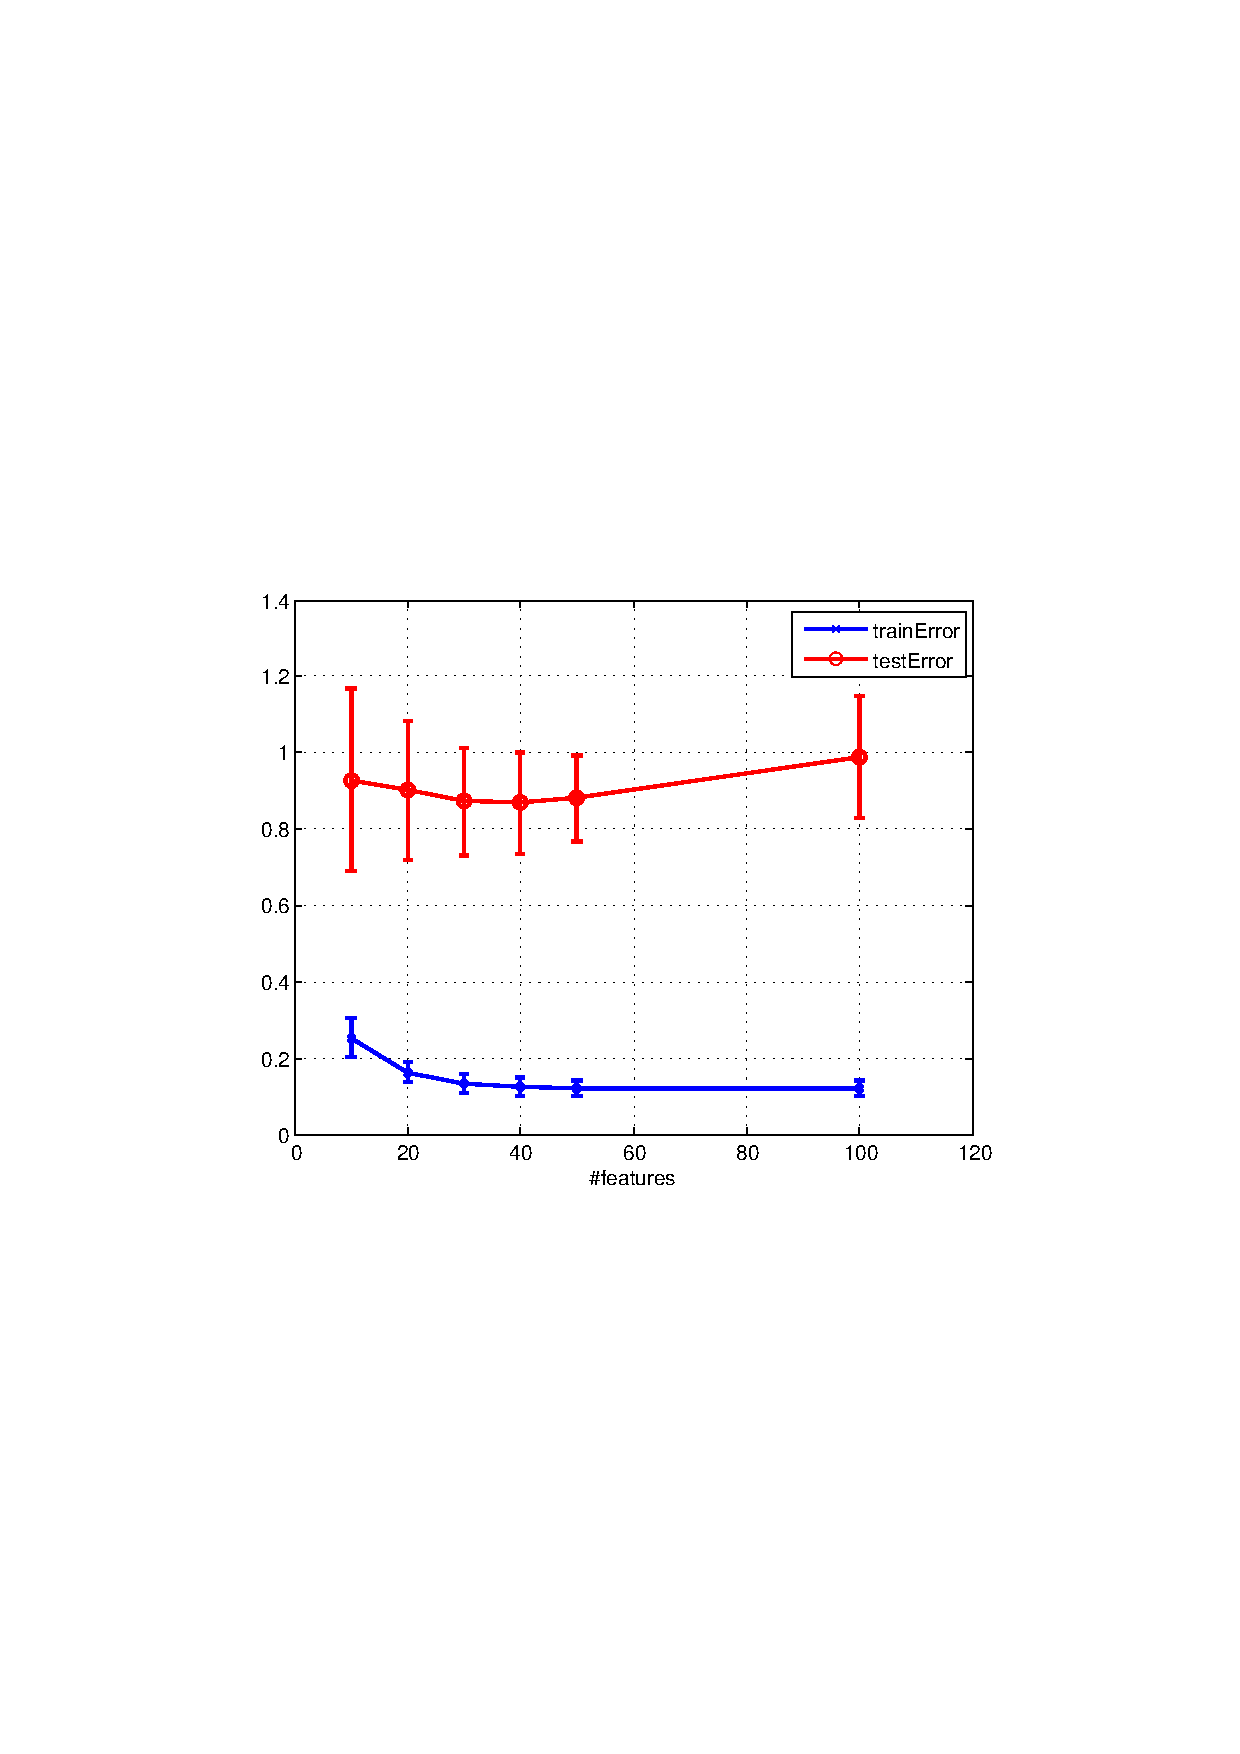
\includegraphics[clip, trim=4cm 9.2cm 3.5cm 9cm, width=\textwidth]{figures/ALS_features.pdf}
    \captionof{figure}{Comparison of Train and Test errors with different features values}
    \label{fig:ALS_features}
    \end{minipage}
  \end{minipage}
  
\begin{minipage}{\textwidth}
  \begin{minipage}[b]{0.45\textwidth}
\begin{center}
  \begin{tabular}{ |l | c | c| }
    \hline
     lambda & MAE train & MAE test \\ \hline
     0.01   & 0.088 ($\pm$  0.0008) &  1.591 ($\pm$ 0.015) \\ \hline
     0.05  &  0.163 ($\pm$  895) &  0.901 ($\pm$  0.0061) \\ \hline
     0.1     & 0.259 ($\pm$ 851)  & 0.822 ($\pm$ 0.0012) \\ \hline
     0.5    & 0.660  ( $\pm$ 851) & 0.864 ($\pm$  0.0016)\\ \hline
     1       & 1.035 ($\pm$ 842) & 1.222($\pm$  0.0010)\\ \hline
     1.5    & 1.493 ($\pm$ 837) & 1.670($\pm$  0.0007) \\
    \hline
  \end{tabular}
  	\label{table:labda_choice}
    \captionof{table}{Estimated Train and Test MAE for the two blob models.}
\end{center}
  \end{minipage}
  \hfill
  \begin{minipage}[b]{0.45\textwidth}
\begin{center}
  \begin{tabular}{ |l | c | c| }
    \hline
     features & MAE train & MAE test \\ \hline
     10   & 0.253 ($\pm$  0.0017) &  0.927 ($\pm$ 0.0080) \\ \hline
     20  &  0.163 ($\pm$  0.0009) &  0.901 ($\pm$  0.0061) \\ \hline
     30     & 0.133 ($\pm$ 0.0009)  & 0.873 ($\pm$ 0.0047) \\ \hline
     40    & 0.124  ( $\pm$ 0.0008) & 0.868 ($\pm$  0.0044)\\ \hline
     50       & 0.121 ($\pm$ 0.0007) & 0.880($\pm$  0.0038)\\ \hline
     100    & 0.122 ($\pm$ 0.0007) & 0.989($\pm$  0.0053) \\
    \hline
  \end{tabular}
  	\label{table:feature_choice}
    \captionof{table}{Estimated Train and Test MAE for the two blob models.}
\end{center}
    \end{minipage}
  \end{minipage}
  
We can see that a value of lambda in the middle is a reaasonable choise, so we selected lambda to be 0.05 for the next experiments.
Our algorithm did a good job training  with a RMSE less than  3 but a bad job on unseen data with RMSE > 3000, meaning it is overfitting 
the training data and incrasing the value of lambda, the regularization parameter did not help.


We notice that the test error across the 10 different splits of the cross validation has values from 2000 to up to 6000. This is an artifact of the high listening counts present in the long tail and the randomness of the split.
\begin{figure}[h]
  \centering
  \begin{subfigure}[b]{0.45\textwidth}
   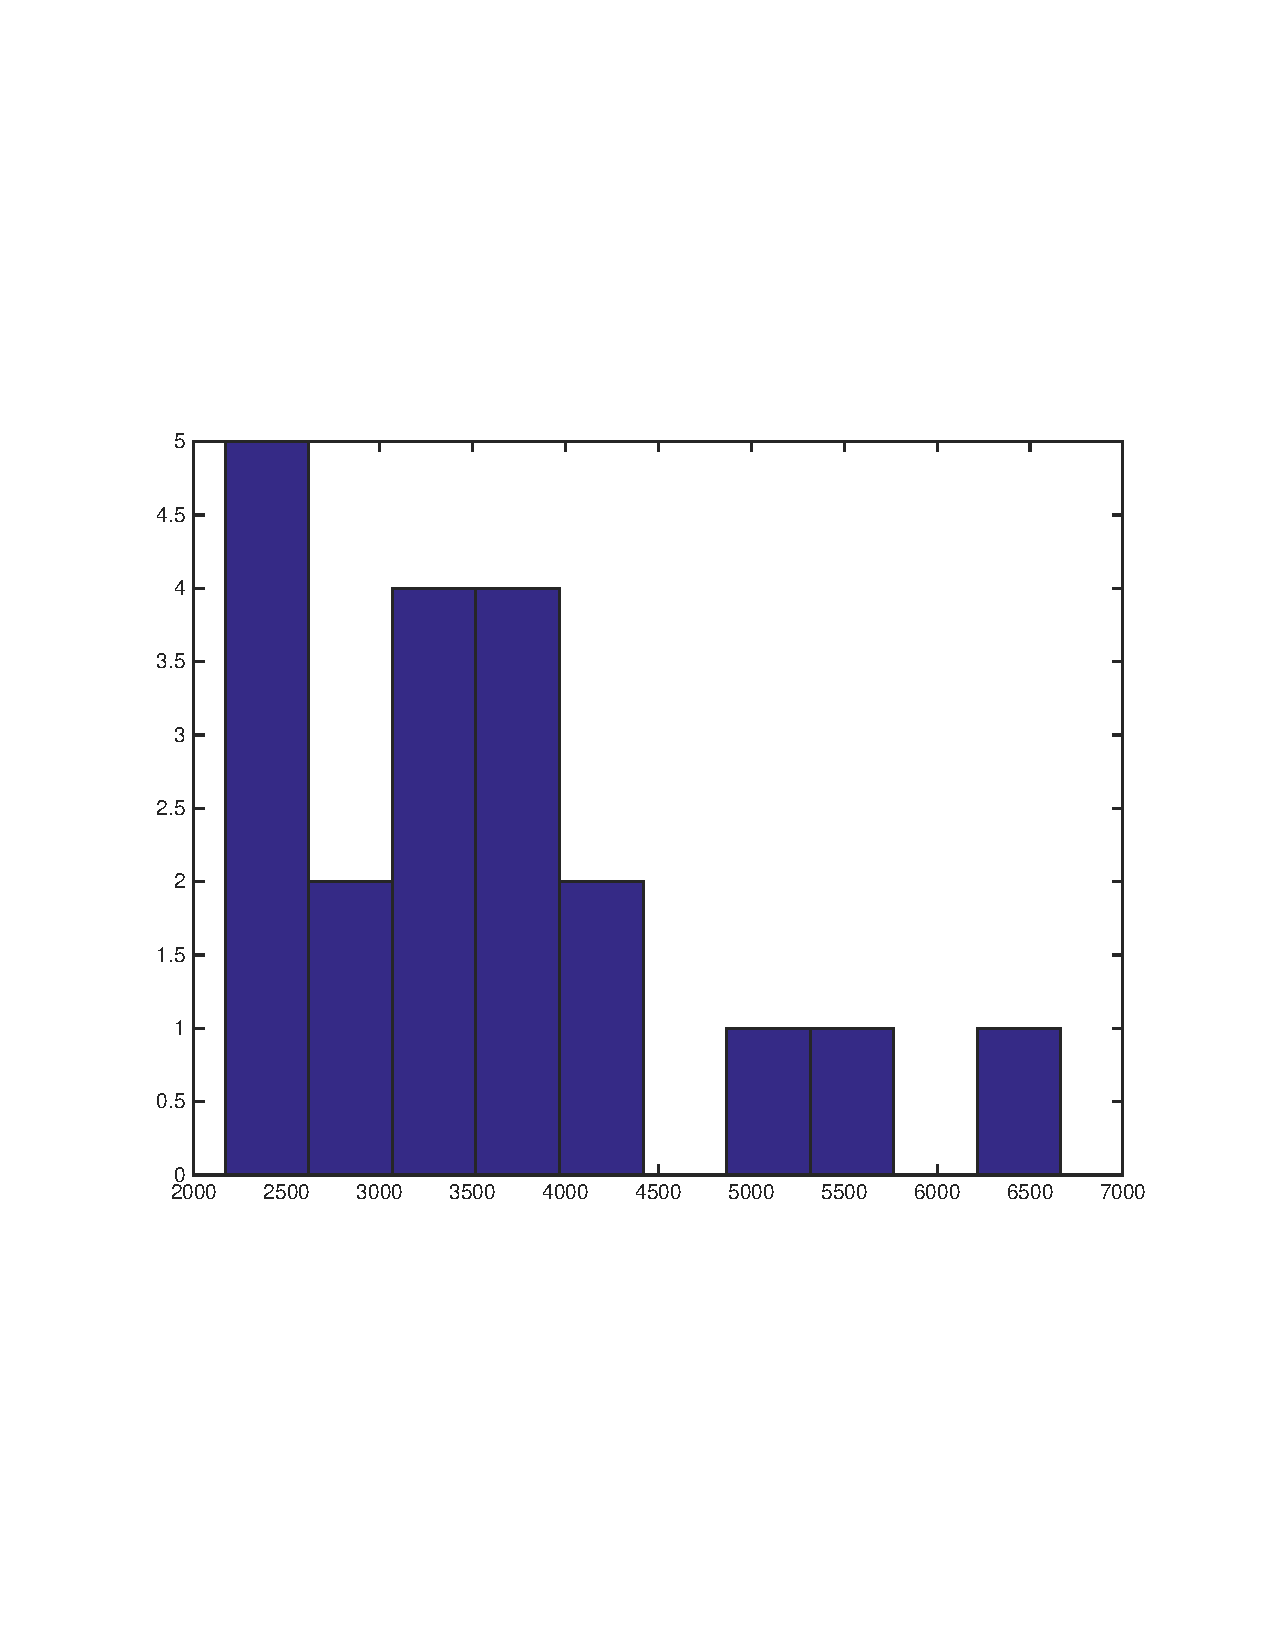
\includegraphics[width=\textwidth]{figures/distributionRMSE.pdf}
    \caption{}
  \end{subfigure}
  \begin{subfigure}[b]{0.45\textwidth}
    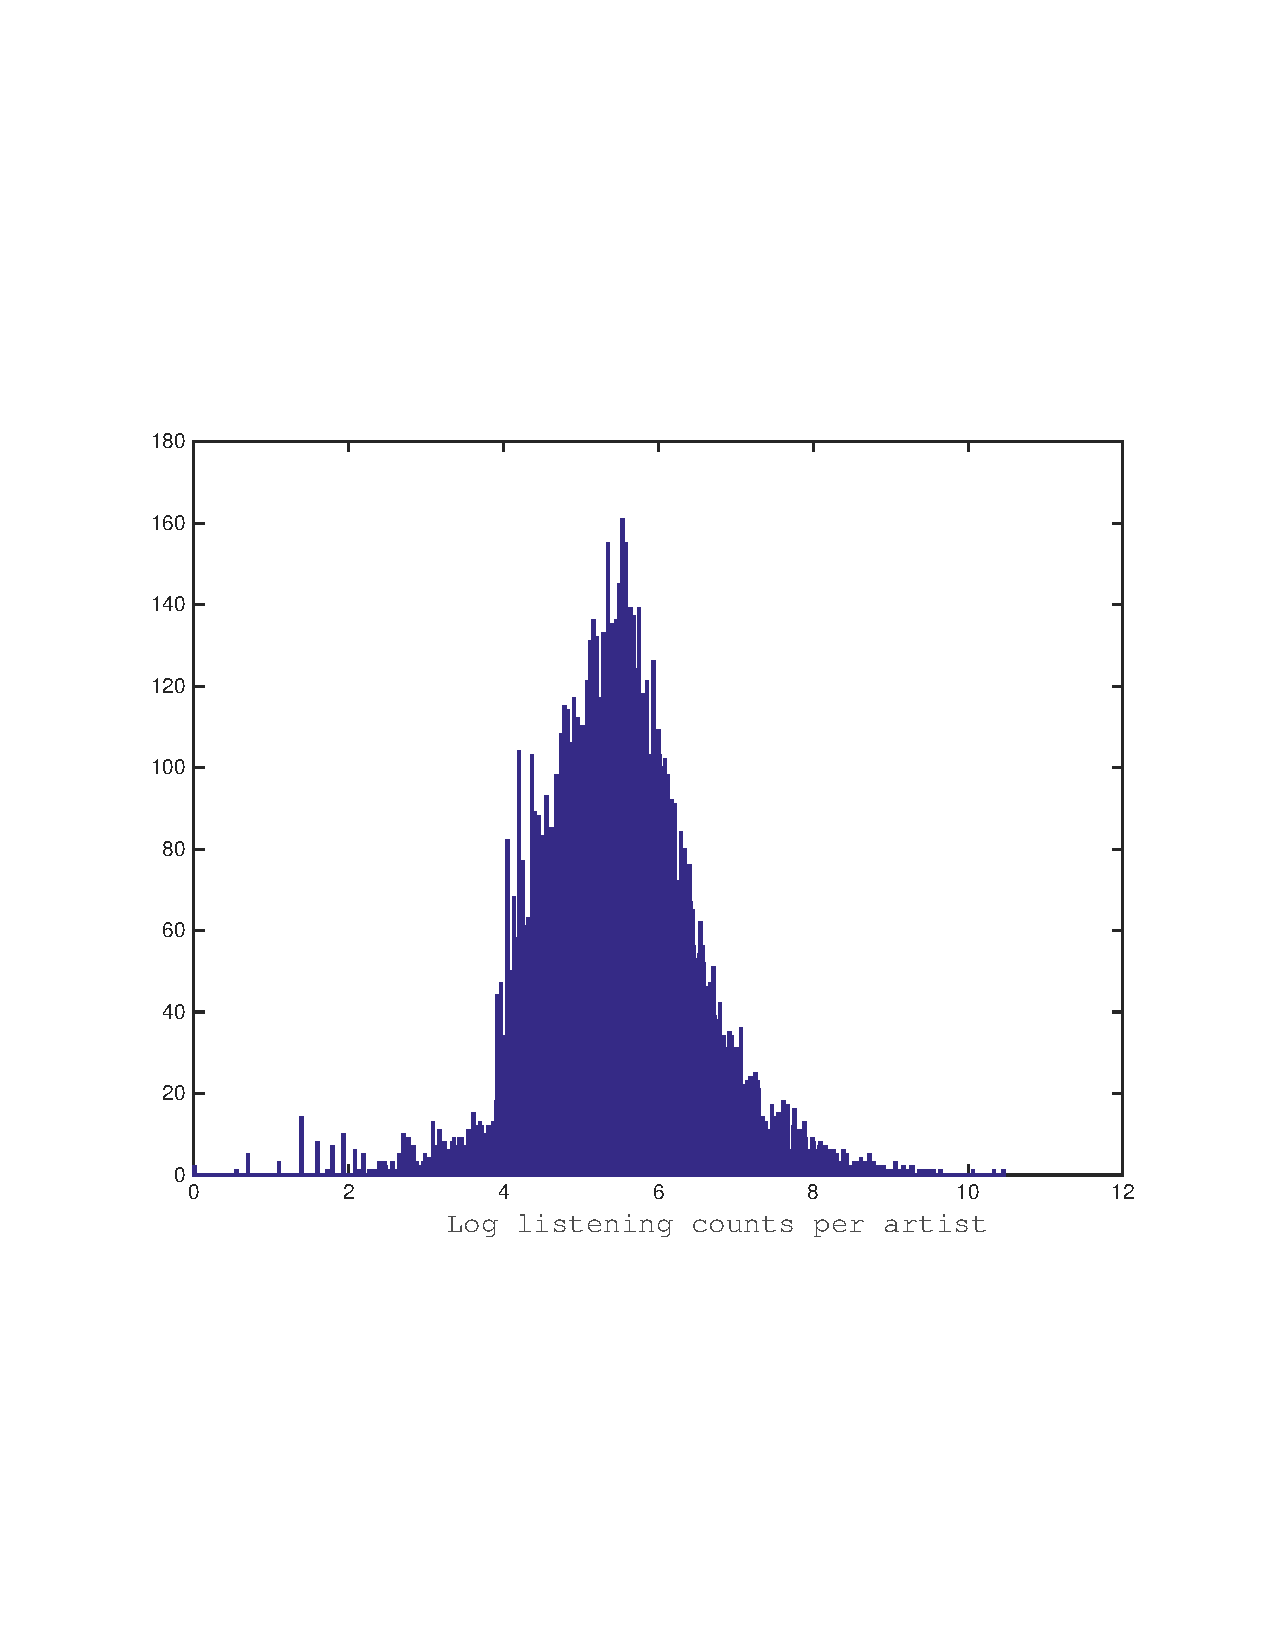
\includegraphics[width=\textwidth]{figures/histCountPerArtist.pdf}
    \caption{}
  \end{subfigure}
  \caption{Distribution per user (a) and per artist(b) log of listenining count distribution}
  \label{fig:new_plot}
\end{figure}

We varied the number of features from 10,20,30,40,50,100 with $\lambda = 0.05$ and repeteated the experiments with different seed.
 Giving train  between 1.24 increasing up to  2.4 for 19 features.  The test RMSE  
 was always in the interval [3569,3546]. None of this results results proved meaningful.

\begin{figure}[h]
  \centering
  \begin{subfigure}[b]{0.45\textwidth}
   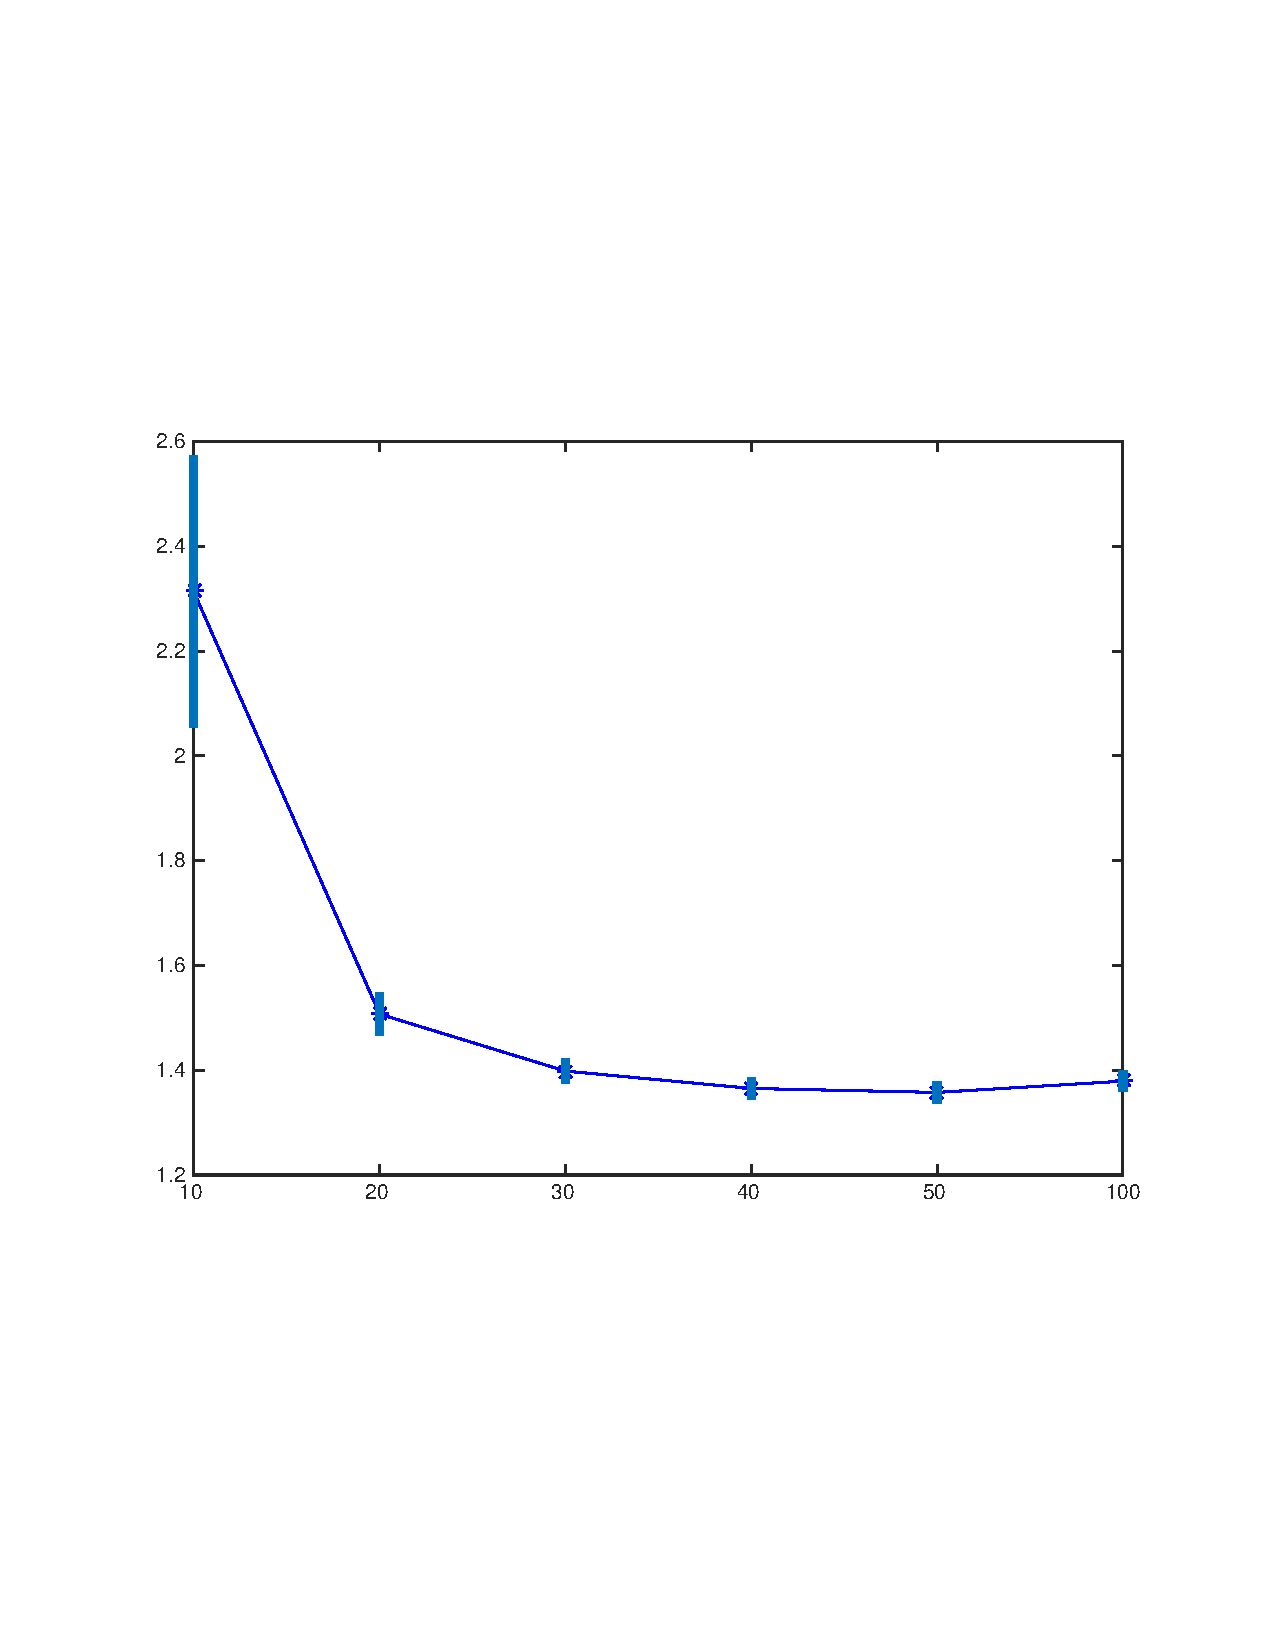
\includegraphics[width=\textwidth]{figures/als_train.pdf}
    \caption{}
  \end{subfigure}
  \begin{subfigure}[b]{0.45\textwidth}
    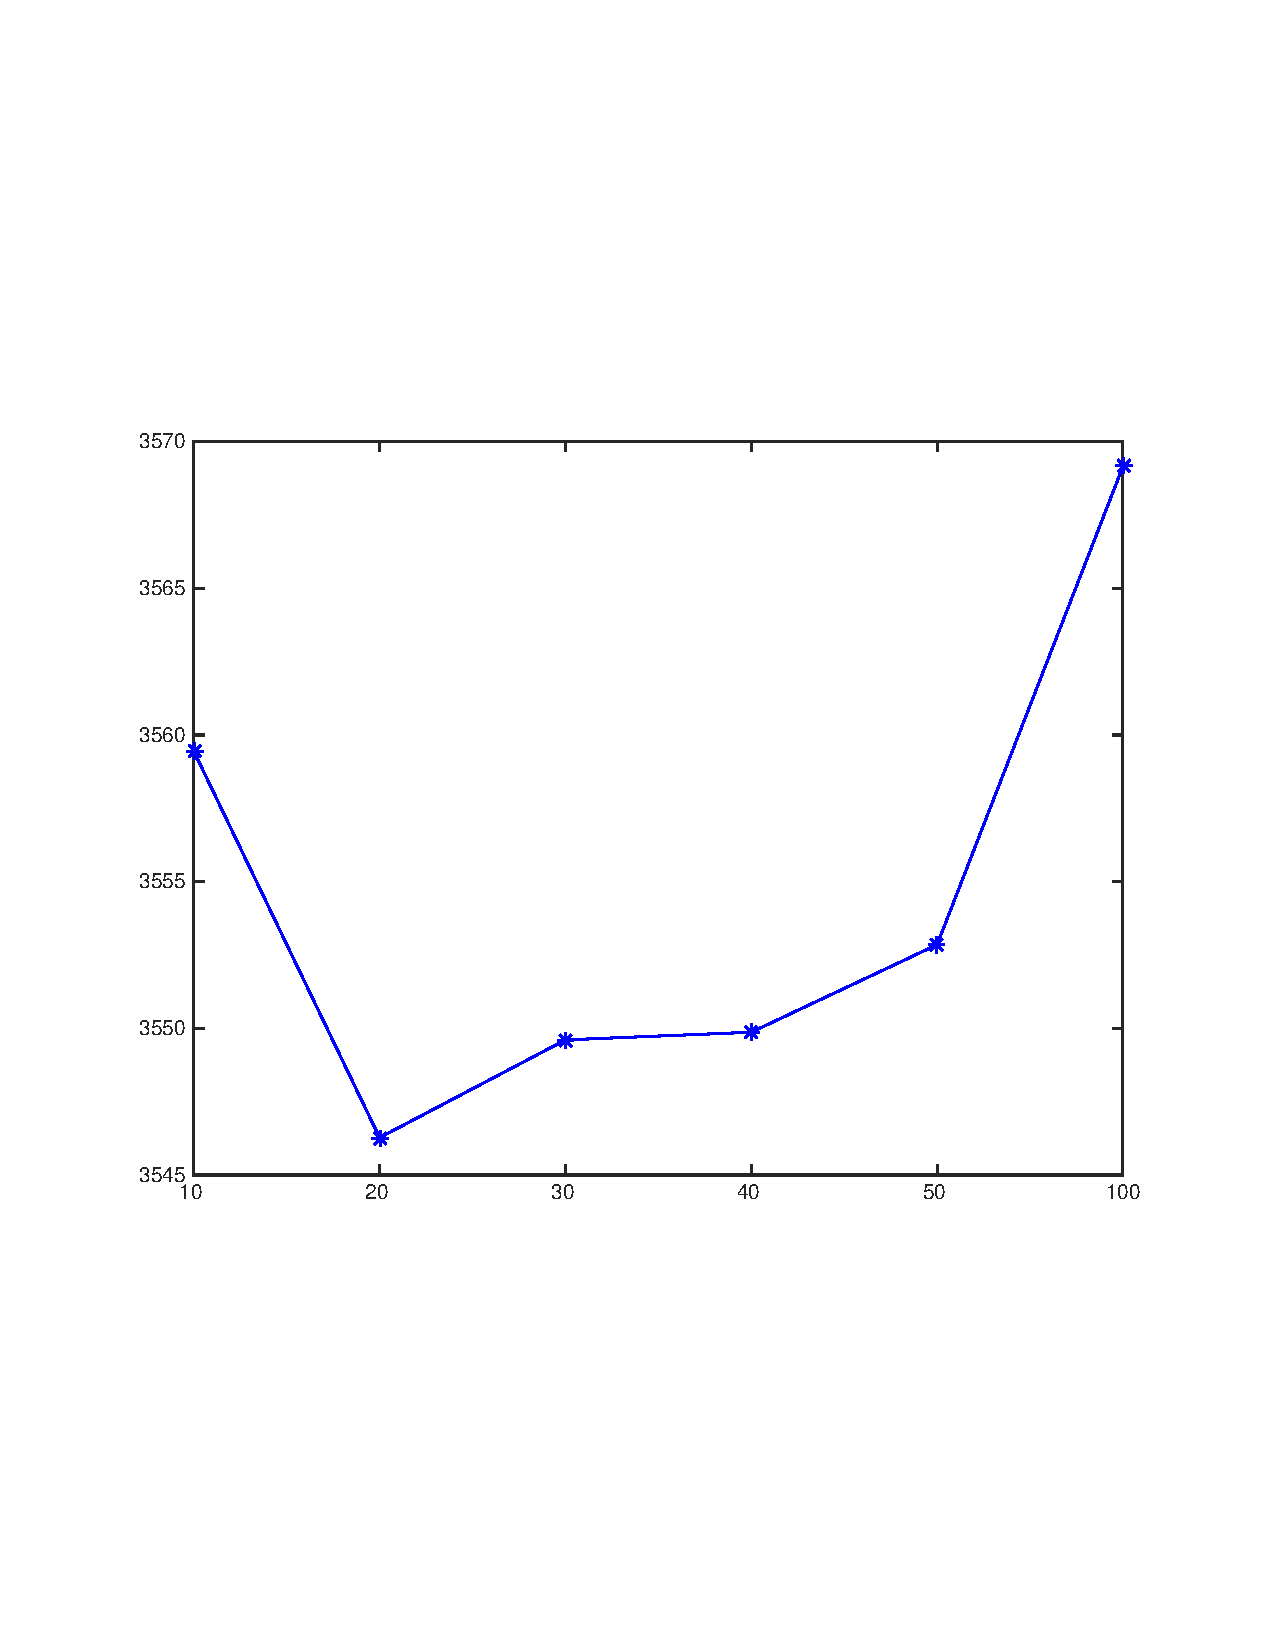
\includegraphics[width=\textwidth]{figures/als_test.pdf}
    \caption{}
  \end{subfigure}
  \caption{Train and Test RMSE for logALS with varying number of features}
  \label{fig:new_plot}
\end{figure}

\subsubsection{Kmeans}
Although the number of artists is 10 times larger than the number of users,
we chose to implement Kmeans with clustering of users 
instead of artists so that we can use the clusters obtained here also in Task 2.

The missing entries in the matrix were initialized with the user average, although that did not have a huge impact on our results. We then sorted the users according to their average score and initialized the clusters with equally spaced samples from the sorted users array. The goal of this cluster initialization was to have a more equilibrated assignment of users to clusters and to make sure we have clusters from both highly active users and also from the less active.

Inspired by the friendship graph information, we tried Kmeans with
varying values from [3,10,20,30,40,50,100]. We plot the mean train and test error using 10 fold cross validation in Fig \ref{fig:kmeans_final}. Using only 3 clusters both the train and the test error was high, while for 100 clusters the difference between train and test error became larger, giving signs of overfitting.

We noticed also the fact that sometimes the training error of Kmeans
(reported by taking exp of data and RMSE) had small fluctuations and it was not always decreasig as the algorithm convergence properties would expect. This is due to the fact that Kmeans miminizes squared error but our cost is a little different since we transform the data using exp.

\begin{figure}[h]
  \centering
  \begin{subfigure}[b]{0.45\textwidth}
   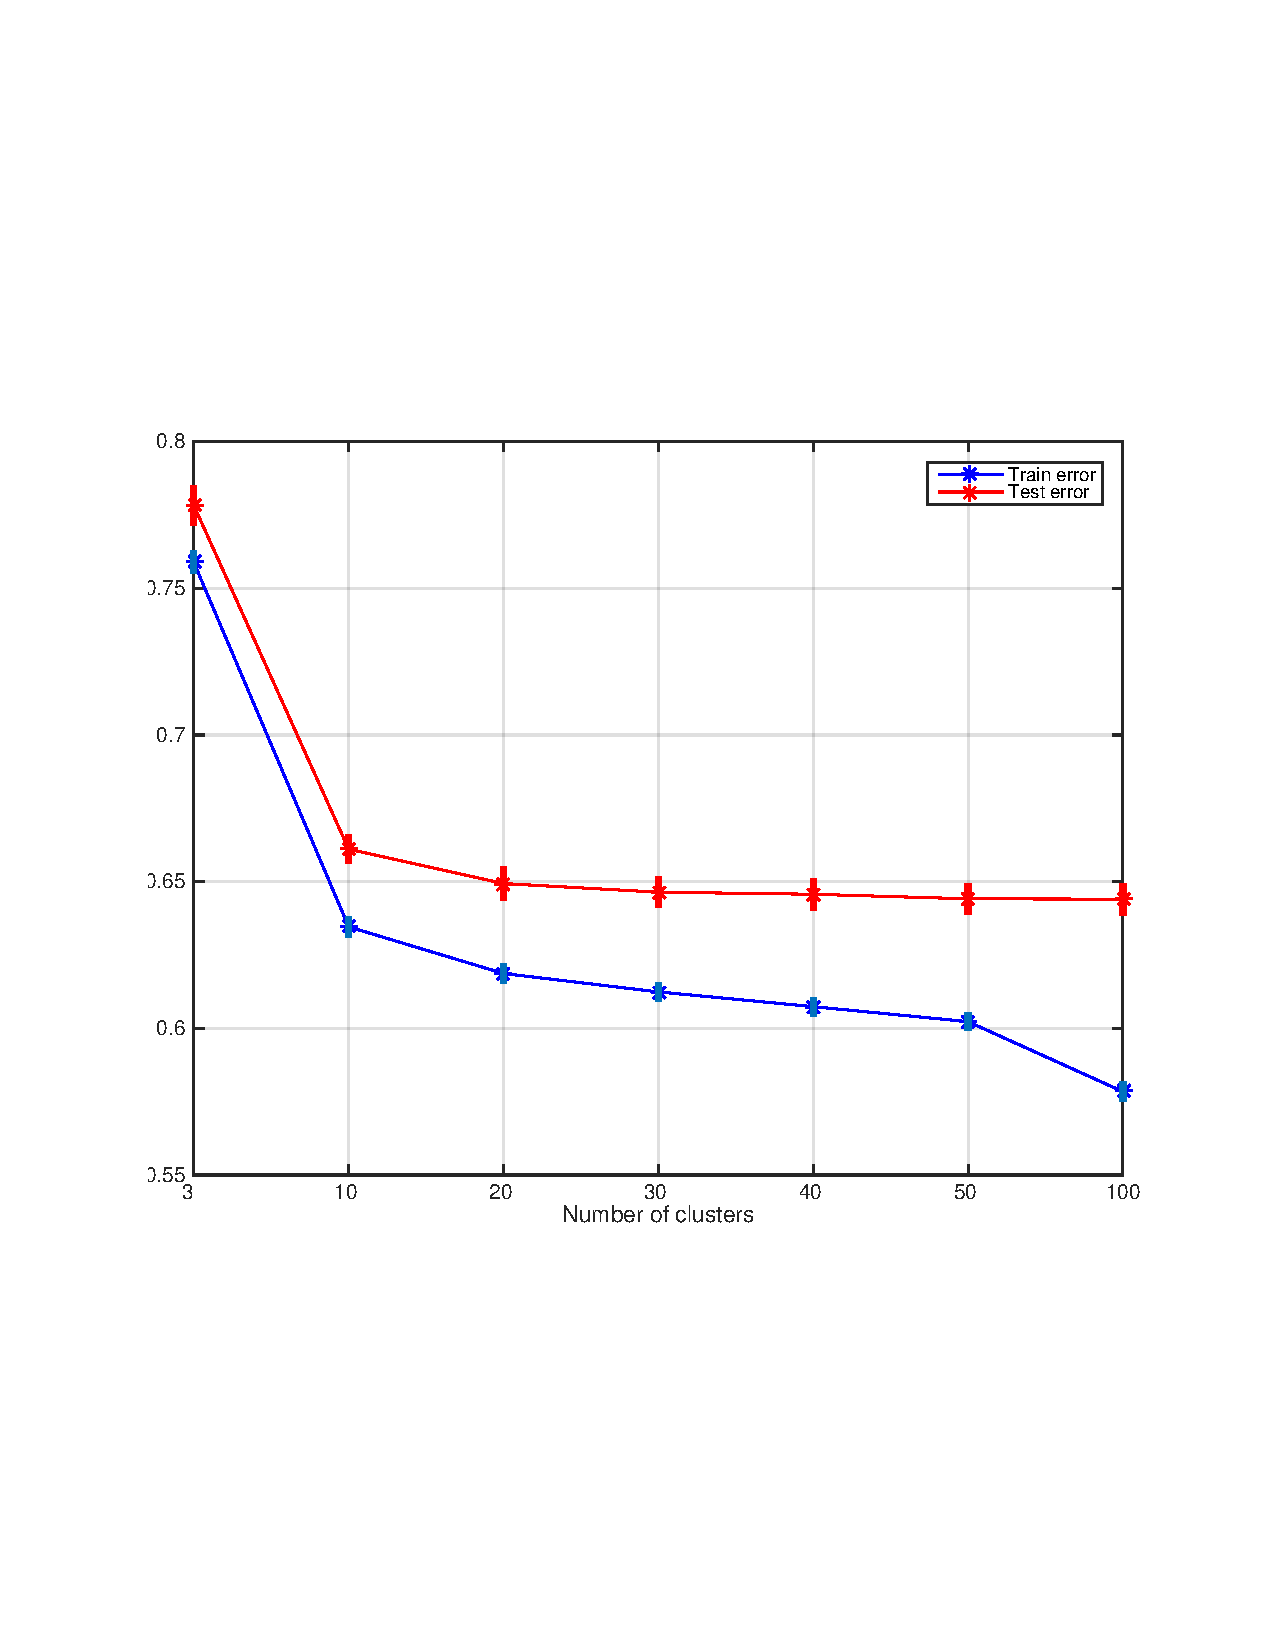
\includegraphics[width=\textwidth]{figures/kmeans_train_test.pdf}
    \caption{}
  \end{subfigure}
  \begin{subfigure}[b]{0.45\textwidth}
    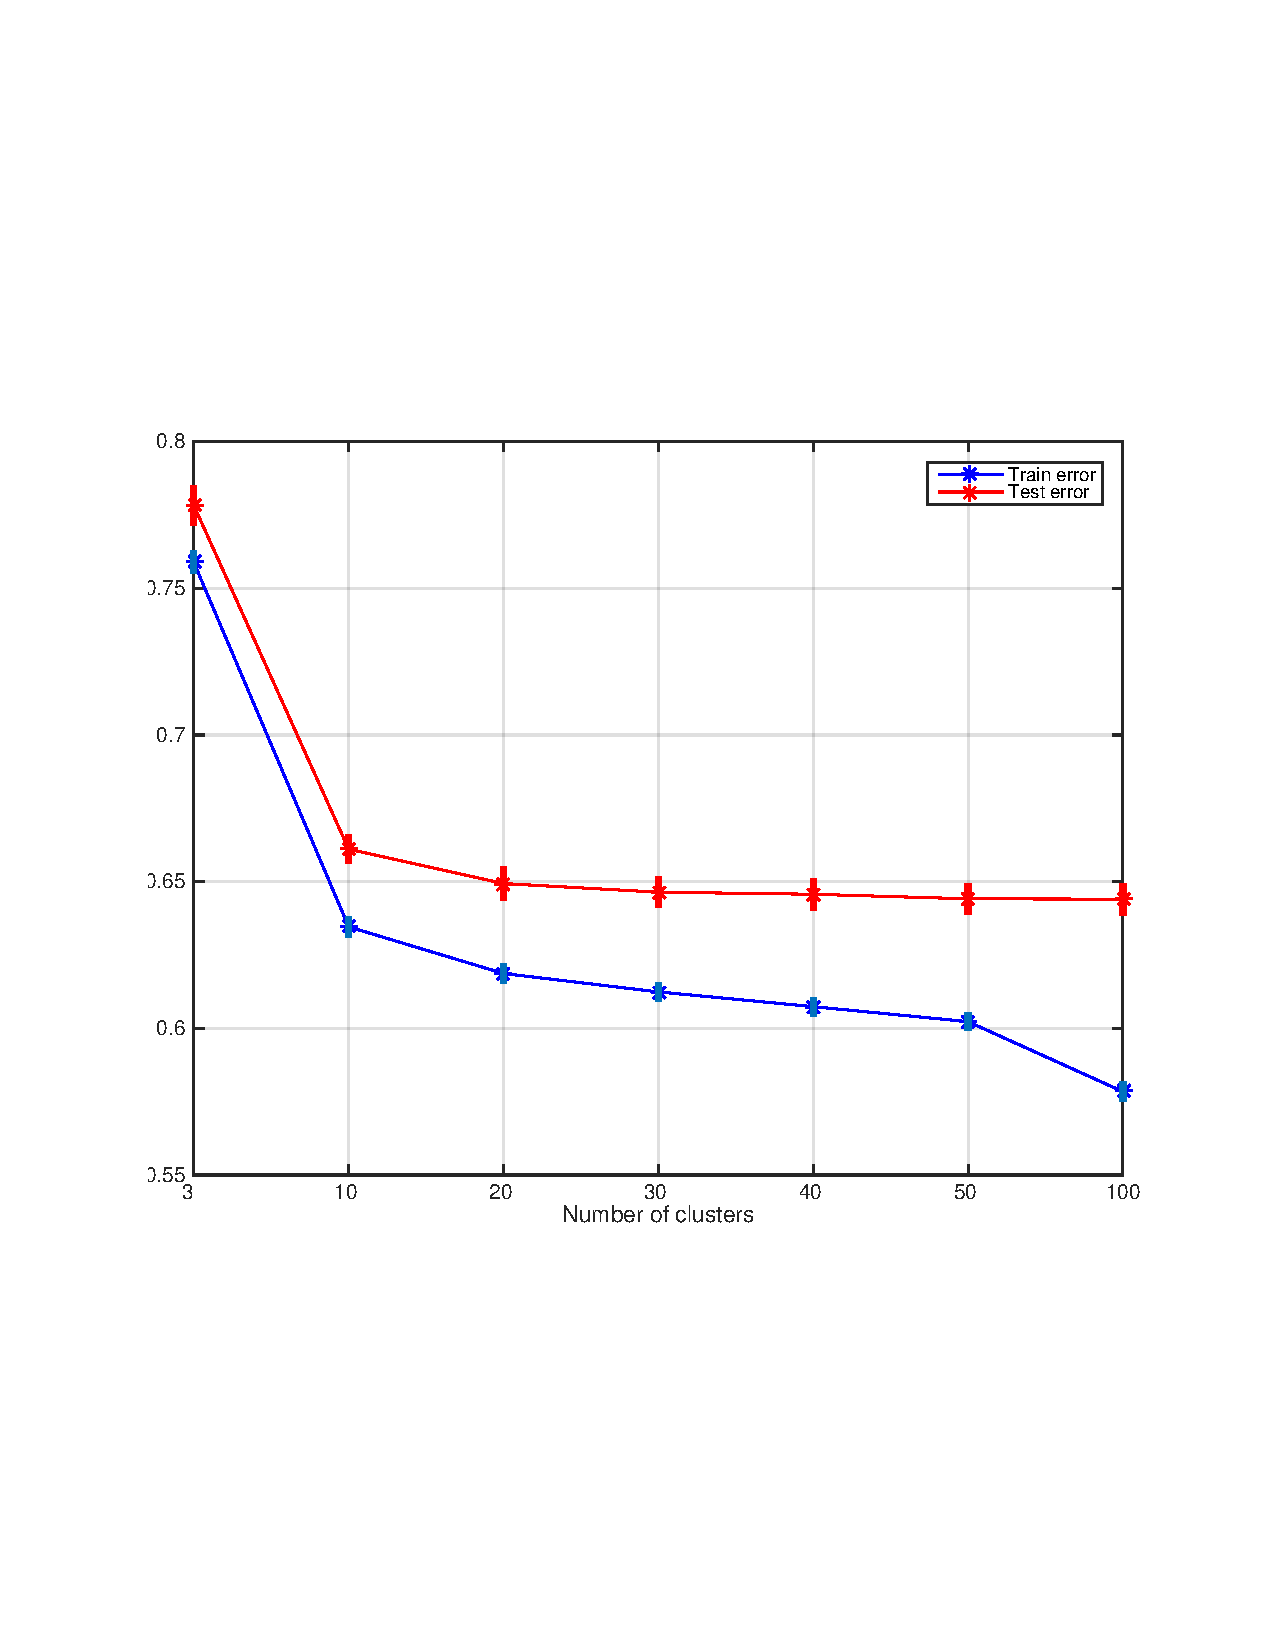
\includegraphics[width=\textwidth]{figures/kmeans_train_test.pdf}
    \caption{}
  \end{subfigure}
  \caption{bla bla}
  \label{fig:kmeans_final}
\end{figure}

In all the experiments with more than 20 clusters obtained a test MAE close to 0.64,.
This was our best test MAE so far. 
For computational reasons, we picked 20 clusters for the next task.

We also tried KMeans where in the update step, only the entries for artists that were known were updated. We expected this to perform better, but the algorithm had problems with overfitting, always giving a train error less than 0.4 (much less than the normal Kmeans) but a test error a bit over 0.7 (higher than the normal KMeans). This happened for all the cluster sizes we experimented with.

\subsection{Task 2}
In this task we make predictions for a set of new users using their friendship information with a set of old users for which partial listening history is available. In other words, we try to see if there is a correlation between
users' friendship and users' preference in music.

\subsubsection{Friendship information}
The initial friendship graph $Gtrain$ of $1776$ nodes and $22904$ edges contained $22$ connected components, but the majority of the components contained just a few nodes.
Using the Gephi  \footnote{http://gephi.github.io/} tool we were able to find some properties of the graph such as the number of communities, 32.  Out of these 32 communities, only 8 communities had more than 150 members.
These statistics were run so that we get an idea of the number of friendship clusters present. The number of connected components and of communities are similar with our choice of 20-30 clusters in KMeans .

We have tried two approaches using the friendship information, one based on the mean average per user and one based on kmeans clustering of users.

\subsubsection{Baseline Methods}
As a reference method, we predict for a missing value the global average of all the available counts, which gave us a MAE of 1.078($\pm$0,044). Taking the average per artist gave us a MAE of 1.767($\pm$  0.09), significantly worse than the above.

\subsection{Average Friend Method}
We sum up this approach as "You are the average of your friends".
In mathematical terms, a prediction for a new user $Ystrong(u,a)$ is computed as the average count of its friends'listening counts $Ytrain(f,a)$ for that artist or global average count for an user without friends (sad).

\begin{table}[h]
  \centering
  \begin{tabular}{ c  l }
  $Ystrong(u,a) $&= $\frac{\sum_{f\in Friends(u), Ytrain(f,a)\neq0}{Ytrain(f,a)}}{n\_fa}, n\_fa \neq 0$ \\ 
                          &= $global\_average, n\_fa = 0$ \\ 
  \end{tabular}
\end{table}
where $n\_fa$ is the cardinality of the set $\left\{ Ytrain(f,a)\neq0, f\in Friends(u)\right\}$

For this setup  we obtain  1.52 ($pm$0.291) which is smaller than our global average baseline prediction.
If we also take into account the friends of the friends of user u we obtain  a MAE of 1.08($\pm$ 0.041). This result is comparable with the global average result.

\subsubsection{KMeans}
We cluster the users into 20 groups using the KMeans setup from Task 1
and repeat the experiments. For a new user, we predict the count as the  mean of its friends' cluster. This gave us a MAE of
1.08($\pm$ 0.04). This is similar with the best prediction from the above approach and with the baseline global average. 
Although KMeans with 20 features behaves similar with the baseline global average, we decided to use this on our newly predicted data.

We mention that we had other unsuccessful experiments where the clusters were updated with the mean of the unique values or using only the most common cluster (test MAE = 1.49), KMeans with 100 clusters (test MAE = 1.55). Same results obtained with 30 friends.

\subsection{Summary}
Skwes the results, it is more important to have correct predictions on the users with hight counts. Looking back, we could have kep track of the max and median value of the test error to asses the accuracy of our results.
